\newpage
% \section*{Executive Summary}

% \refstepcounter{section}
%Add Image
\vspace*{-40mm} %Make image have no top margin
\begin{tikzpicture}
\node[inner sep=0pt] (x) at (0,0)
    {\hspace{-87mm}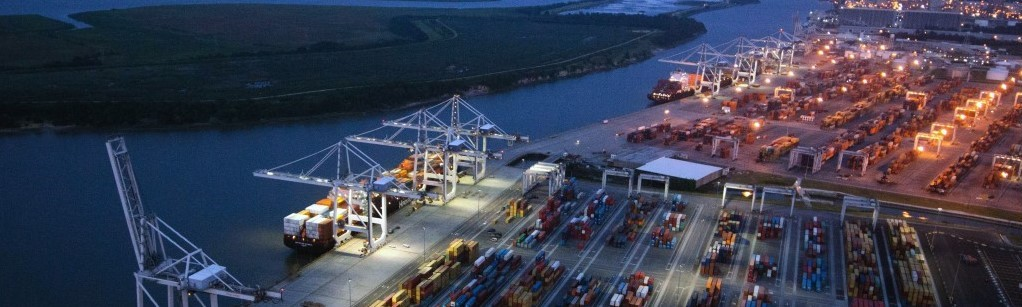
\includegraphics[width=\paperwidth]{sectionimage2.jpg}};
% \node[text width=10in] (Z) at (0,-1) {\color{white}\headingfont\Large\bfseries\uppercase{\hspace{-0.7cm}\thesection\hspace{0.5cm}Executive Summary}};
\node[text width=10in] (Z) at (0,-1) {\color{white}\headingfont\Large\bfseries\uppercase{\hspace{-0.7cm}Executive Summary}};
\end{tikzpicture}
%Modify TOC
% \addcontentsline{toc}{section}{\protect\numberline{\thesection}Executive Summary}
%   \sectionmark{Executive Summary}
\vspace{1.5mm}
% \\This report outlines the feasibility study for the potential relocation of the Ports of Auckland (PoA) in the North Island. The New Zealand cabinet has requested 303 Consulting to undertake this study. The PoA is under stress due to the significant freight capacity it continues to handle. With the port soon to be operating at full capacity, further study suggests that if nothing is done soon, the demand for freight goods will outweigh the amount of freight that can be imported and exported. This will not be economically viable for Auckland in the long term. 
% % \vspace{-4mm}
% \\ \newline This study considered the following stakeholder requirements:
% \begin{itemize}[noitemsep]
%     \vspace{-2mm}
%     \item Efficiently transporting freight with the use of existing road and rail networks
%     \item Reduce shipping traffic in PoA and congestion of traffic in wider Auckland
%     \item Determine overall financial feasibility for the proposed solution
%     \item Create economic expansion and opportunities in other areas of the North Island
% \end{itemize}
% Based on the following analysis, the recommended solution is to incrementally relocate shipping traffic to the Port of Tauranga (PoT), while reducing the amount of shipping traffic coming into Auckland. Re-scaling of the ports will take place over a 10 year period. It is proposed that these changes will begin in the year 2025. PoA will be reduced to roughly 20\% of its current operating traffic by the end of the 10 year period, while the PoT will be allowed to expand. 
% \\ \newline Several options were analysed using an iterative process. Unsuitable details were identified and eliminated, narrowing down potential courses of action. As a result, the solution incorporates ideas from a handful of initial options. We came to the conclusion that by maintaining the PoA and relocating some of the shipping traffic to PoT allows PoA to downsize over a number of years. This reduction in size will free up prime real estate on the waterfront, currently being occupied by the PoA and will ease on-road traffic congestion around the port in central Auckland.
% % \vspace{-4mm}
% \\ \newline The decision to build an entirely new port was vetoed as it was found that in order to make that a feasible alternative, significant infrastructure was required to be built in order to support freight traffic alongside the construction of an entirely new port. While this motion was initially attractive, topography surrounding potential sites (including Manukau, Muriwai and Kawakawa Bay) was complex and infrastructure to and from the port was going to be significant and costly. The solution we propose minimises the need to build infrastructure from scratch and utilises the potential for an increase in capacity of pre-existing ports. It also means that shipping routes are not going to be affected in any way as these routes already exist and are currently being used.
% % \vspace{-4mm}
% \\ \newline The infrastructure connecting the various ports will need to be upgraded, the project will make use of the Regional Rapid Rail plan, which will connect the PoA to Hamilton, and then will go to Tauranga. This takes advantage of further establishment of the “Golden Triangle” between Auckland, Hamilton and Tauranga. This will also fund the addition of a new rail from Hamilton to Tauranga and the expansion of the highway between Tauranga and state highway.
\\This report outlines the feasibility study for the potential relocation of the Port of Auckland (PoA). The New Zealand cabinet has requested 303 Consulting to undertake this study. The PoA is under stress due to freight handling nearing capacity. With the port soon to be operating at full capacity; studies suggest that if nothing is done soon the demand for freight will outweigh the amount of freight that can be imported and exported. This is not economically viable in the long term. 
\vspace{-4mm}
\\ \newline This study considered the following stakeholder requirements:
\begin{itemize}[noitemsep]
    \vspace{-2mm}
    \item Efficiently transporting freight with the use of existing road and rail networks
    \item Reduce shipping traffic in PoA and congestion of traffic in wider Auckland
    \item Determine overall financial feasibility for the proposed solution
    \item Create economic expansion and opportunities in other areas of the North Island
\end{itemize}
Based on the following analysis, the recommended solution is to incrementally relocate shipping traffic to the Port of Tauranga (PoT), while reducing the amount of shipping traffic coming into PoA. Re-scaling of the ports will take place over a ten year period. It is proposed that these changes will begin in the year 2025. PoA will be reduced to roughly 20\% of its current operating traffic by the end of this period, while the PoT will be allowed to expand. 
\vspace{-4mm}
\\\newline Several options were analysed using an iterative process. Unsuitable details were identified and eliminated, narrowing down potential options. Based on the analysis, the best solution is maintaining the PoA and relocating some of the shipping traffic to the PoT; allowing PoA to downsize over a number of years. This reduction in size will free up the prime real estate on the waterfront, currently being occupied by the PoA, and will ease on-road traffic congestion in Auckland CBD.
\vspace{-4mm}
\\\newline The decision to build an entirely new port was vetoed due to infeasibility. Significant infrastructure would be required to support freight traffic alongside the construction of an entirely new port. While this motion was initially attractive, topography surrounding potential sites (including Manukau, Muriwai and Kawakawa Bay) was complex and infrastructure to and from the port would be significant and exorbitant. The solution we propose minimises the need to build infrastructure and utilises PoT’s current capacity. 
\vspace{-4mm}
\\\newline The infrastructure connecting the various ports will need to be upgraded. Our proposed solution makes use of the Regional Rapid Rail plan, which will connect the Auckland to Hamilton and finish in Tauranga. This takes advantage of the Governments “Golden Triangle” initiative between Auckland, Hamilton and Tauranga, opening up the opportunity for increased funding for the \$15 billion project. This will also fund the addition of a new rail from Hamilton to Tauranga and the expansion of the main highways connecting to Tauranga.


\clearpage